%%%%%%%%%%%%%%%%%%%%%%%%%%%%%%%%%%%%%%%%%%%%%%%%%%%%%%%%%%%%%%%%%%%%%%
% problem statement
\begin{statement}[
  problempoints=50,
  timelimit=1 second,
  memorylimit=512 MiB,
]{Trol}

\setlength\intextsep{-0.1cm}
\begin{wrapfigure}[11]{r}{0.22\textwidth}
\centering
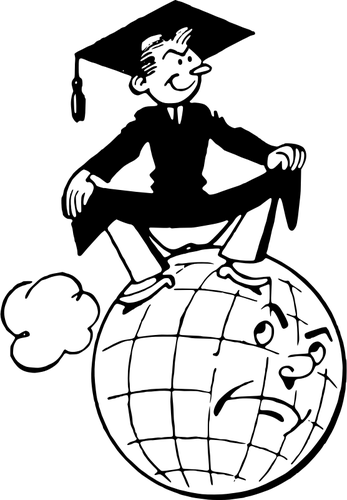
\includegraphics[width=0.22\textwidth]{img/diploma.png}
\end{wrapfigure}

%\subsection

Stjepan recently received his bachelor's degree in mathematics from the
University of Zagreb. Naturally, his parents are very proud and have decided
to give him all positive integers not greater than $2^{60}$ as a gift. To keep
them safe, he quickly stored all of those numbers in an array $A$, such that
$A_i = i$.

His jealous friend Marin decided to prank him by repeatedly replacing each
element of $A$ with the sum of its digits until all elements of $A$ consisted
of a single digit. For example, the initial value of $197$\textsuperscript{th}
element of $A$ was $197$. Marin first changed that value to $1 + 9 + 7 = 18$ and
then changed its value again to $1 + 8 = 9$.

Stjepan is devastated and begs Marin to return his array to its initial state.
Unfortunately, Marin won't do that until Stjepan correctly answers his $Q$
queries: ``What is the sum of numbers from $l$-th to $r$-th element of $A$''.

Help Stjepan answer those queries!

%%%%%%%%%%%%%%%%%%%%%%%%%%%%%%%%%%%%%%%%%%%%%%%%%%%%%%%%%%%%%%%%%%%%%%
% Input
\subsection*{Input}
The first line contains an integer $Q$ $(1 \le Q \le 100)$ from the task
description. \\
The next $Q$ lines contain two integers $l_i$ i $r_i$
$(1 \le l_i \le r_i \le 2^{60})$, the parameters of Marin's $i$-th query.

%%%%%%%%%%%%%%%%%%%%%%%%%%%%%%%%%%%%%%%%%%%%%%%%%%%%%%%%%%%%%%%%%%%%%%
% Output
\subsection*{Output}
Output the answers to each of Marin's $Q$ queries. Each answer should be
printed in a separate line and their order should match the order of the
queries as they are given in the input.

%%%%%%%%%%%%%%%%%%%%%%%%%%%%%%%%%%%%%%%%%%%%%%%%%%%%%%%%%%%%%%%%%%%%%%
% Scoring
\subsection*{Scoring}
In test cases worth a total of $10$ points, for each query will hold
$1 \le l_i \le r_i \le 9$. \\
In test cases worth a total of $30$ points, for each query will hold
$r_i - l_i \le 1000$.

%%%%%%%%%%%%%%%%%%%%%%%%%%%%%%%%%%%%%%%%%%%%%%%%%%%%%%%%%%%%%%%%%%%%%%
% Examples
\subsection*{Examples}
\begin{tabularx}{\textwidth}{X'X'X}
\sampleinputs{test/trol.dummy.in.1}{test/trol.dummy.out.1} &
\sampleinputs{test/trol.dummy.in.2}{test/trol.dummy.out.2} &
\sampleinputs{test/trol.dummy.in.3}{test/trol.dummy.out.3}
\end{tabularx}

\textbf{Clarification of the second example:}

\textbf{1\textsuperscript{st} query} \textrightarrow{}
$A_9 = 9$, $A_{10} = 1 + 0 = 1$, $A_{11} = 1 + 1 = 2$,
$A_{12} = 1 + 2 = 3$, $A_{13} = 1 + 3 = 4$.\\
\phantom{\textbf{1\textsuperscript{st} query} \textrightarrow{}}
$A_9 + A_{10} + A_{11} + A_{12} + A_{13} = 9 + 1 + 2 + 3 + 4 = 19$.

\textbf{2\textsuperscript{nd} query} \textrightarrow{}
$A_{44} = 4 + 4 = 8$, $A_{45} = 4 + 5 = 9$. $A_{44} + A_{45} = 8 + 9 = 17$.

%%%%%%%%%%%%%%%%%%%%%%%%%%%%%%%%%%%%%%%%%%%%%%%%%%%%%%%%%%%%%%%%%%%%%%
% We're done
\end{statement}

%%% Local Variables:
%%% mode: latex
%%% mode: flyspell
%%% ispell-local-dictionary: "croatian"
%%% TeX-master: "../hio.tex"
%%% End:
